\section{Durchführung} \label{sec:durchführung}

Im Folgenden soll hier die Durchführung des Versuchs beschrieben werden.

\subsection{Aufbau}

    Die Messung der Wärmeleitfähigkeit wird mithilfe einer Platte, auf der die Metalle
    Aluminium, Edelstahl und zweimal Messing in Form von Stäben befestigt sind.
    Ein Peltierelement in der Mitte der Platte heizt oder kühlt die Stäbe.
    Für diese Einstellung ist ein Schalter mit den Optionen $"HEAT"$ und $"COOL"$ gegeben.
    An die Platte ist eine Spannung $U_\text{P}$ angeschlossen, sodass das Peltierelement mit maximalem
    Strom versorgt wird.
    
    %TODO Aufbau einfügen, funktioniert hier nicht wie gewollt.
    %\begin{figure}
    %    \centering
    %    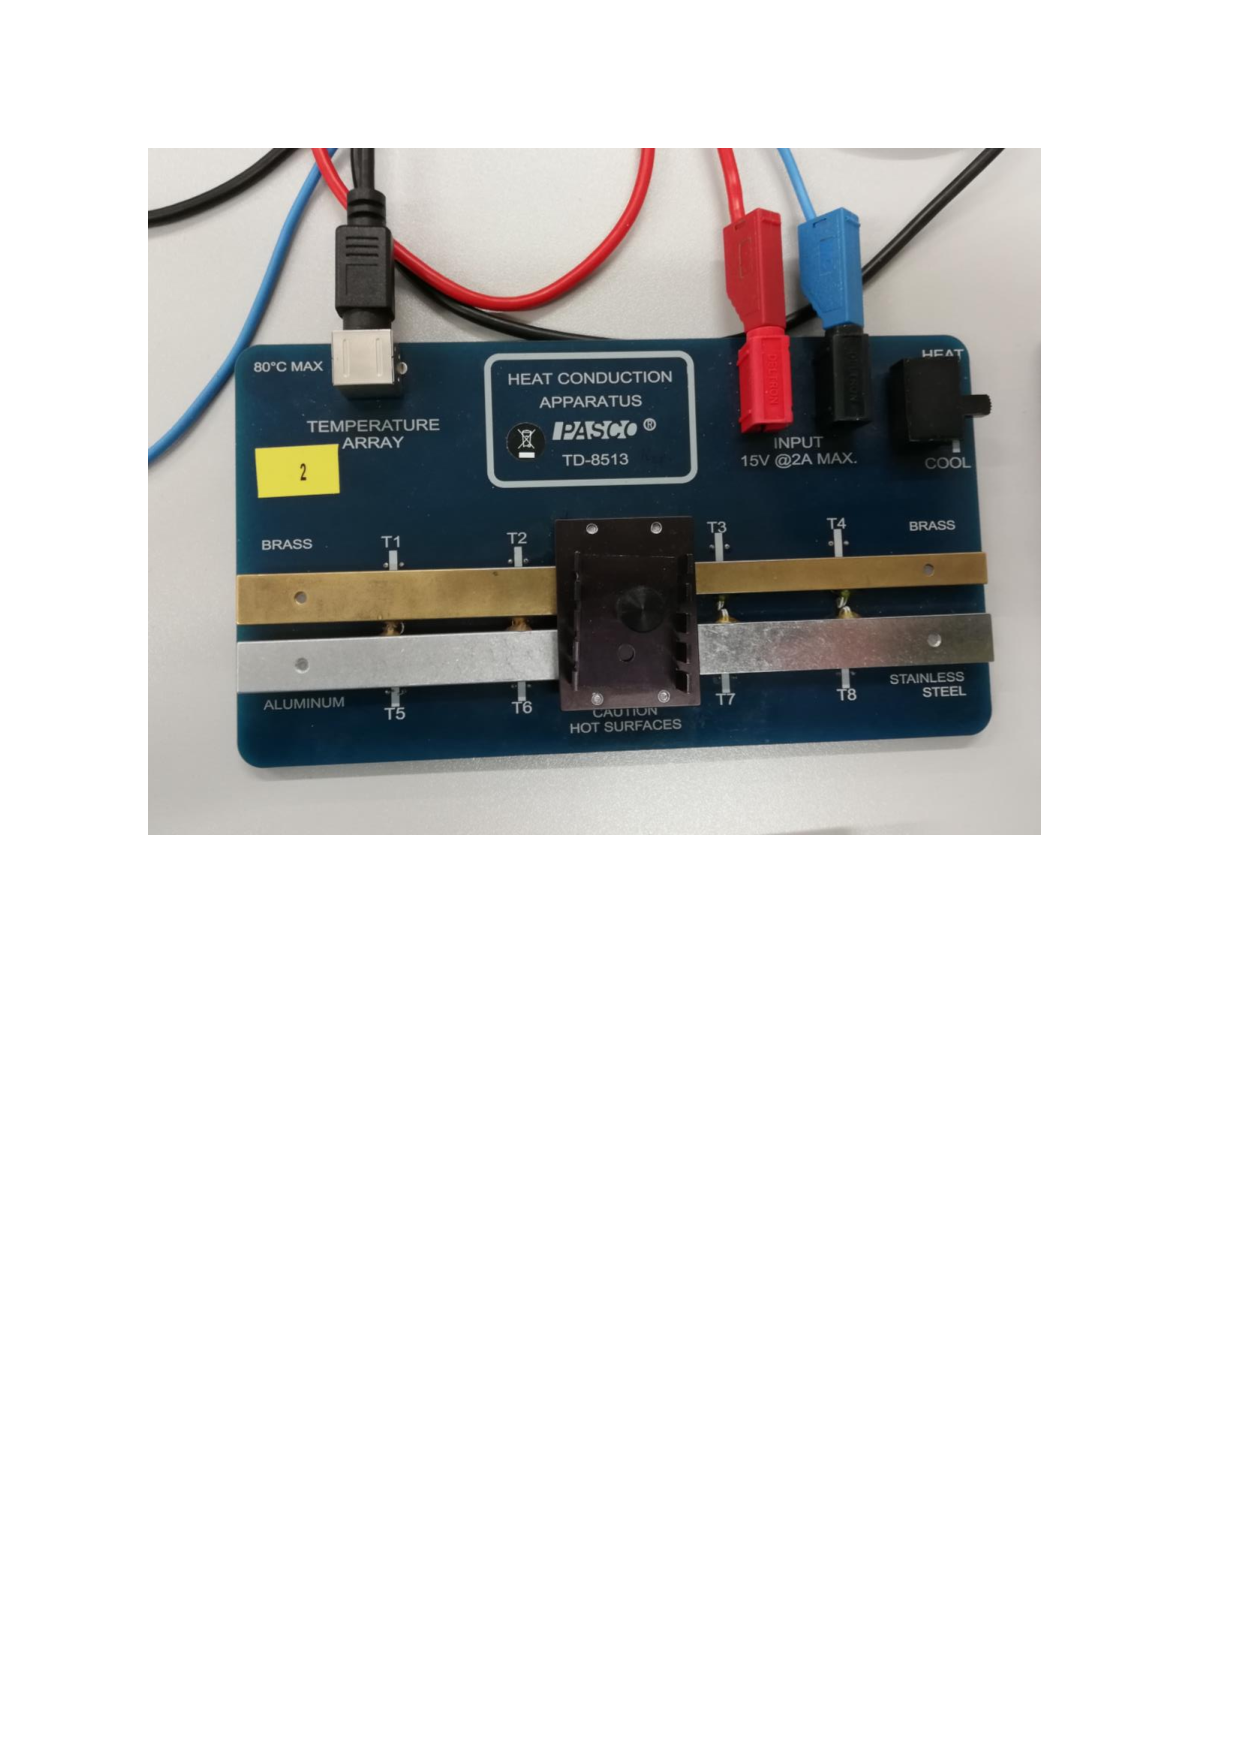
\includegraphics{foto_aufbau.pdf}
    %    \caption{Aufbau der Grundplatte}
    %    \label{fig:aufbau}
    %\end{figure}

    Die Thermoelemente T1 und T2 befinden sich am breiten Messingstab, die Elemente
    T3 und T4 am schmalen Messingstab.
    Am Aluminiumstab befinden sich T5 und T6, am Edelstahlstab T7 und T8.
   
    Für die Abmessungen der Stäbe sind folgende Werte gegeben.
    \begin{table}
        \centering
        \caption{Eigenschaften der Metallstäbe.}
        \label{tab:vorgegebeneDaten}
        \begin{tabular}{c c c c}
            \toprule
            $Material$ & $Abmessungen[cm]$ & $\rho [\frac{kg}{m^3}]$ & $c [\frac{J}{kg \cdot K}]$ \\
            \midrule
            Messing(breit) & 9 x 1.2 x 0.4 & 8520 & 385 \\
            Messung(schmal) & 9 x 0.7 x 0.4 & 8520 & 385 \\
            Aluminium(breit) & 9 x 1.2 x 0.4 & 2800 & 830 \\
            Edelstahl(breit) & 9 x 1.2 x 0.4 & 8000 & 400 \\
            \bottomrule
        \end{tabular}
    \end{table}

    Zur Aufnahme der Messwerte ist ein GLX Datenlogger "Xplorer GLX" gegeben.
    Dieser wird so eingestellt, dass alle acht Temperaturen der Thermoelemente angezeigt werden.\\

    Während der Messung muss eine Wärmeisolierung über die Stäbe gelegt werden,
    damit möglichst wenig Wärmeaustausch zwischen den Stäben und der Umgebung stattfinden kann.
    Nach jeder Messung werden die Stäbe bis auf eine Temperatur von $\SI{30}{\celsius}$ oder 
    weniger gekühlt, bevor eine neue Messung gestartet werden kann.

\subsection{Die statische Methode}

    Bei der statischen Methode wird die Temperatur an den Thermoelementen bei 
    laufender Zeit gemessen.
    Zunächchst wird der Abstand $x$ zwischen den Thermoelementen gemessen.
    Die angelegte Spannung $U_\text{P}$ wird auf $\SI{5}{\volt}$ eingestellt.
    Am Xplorer wird eine Abtastrate $\symup{\Delta} t_\text{GLX} = \SI{5}{\second}$ eingegeben.
    Zum Messen des Temperaturverlaufs wird die Isolierung auf die Stäbe gelegt und der Schalter auf $"HEAT"$ gestellt.
    Die Messung wird solange geführt, bis das Thermoelement T7 eine Temperatur von ungefähr $\SI{45}{\celsius}$ hat.
    Zudem werden nach $\SI{700}{\second}$ die Temperaturen der Elemente T1, T4, T5 und T8 aufgeschrieben, um 
    zu prüfen, welches Material die beste Leitung besitzt.
    Nach Beenden der Messung werden die Stäbe gekühlt, in dem der Schalter auf $"COOL"$ gestellt wird.
    Währenddessen werden die aufgenommenen Messdaten des Xplorers gesichert.
    %Die Wärmeleitfähigkeit soll aus dem Temperaturverlauf berechnet werden.

\subsection{Die dynamische Methode}

    Die dynamische Methode wird auch Angström-Messverfahren genannt.
    Bei dieser Methode werden die Stäbe periodisch erhitzt und gekühlt.
    %Die Wärmeleitfähigkeit kann mithilfe der entstehenden Temperaturwelle berechnet werden.
    Die Spannung $U_\text{P}$ wird bei dieser Methode auf einen Wert von $\SI{8}{\volt}$ eingestellt
    und die Abtastrate des Xplorers auf $\symup{\Delta} t_\text{GLX} = \SI{2}{\second}$.
    Es werden zwei Messungen durchgeführt.\\
    Bei der ersten Messung wird mit einer Periodendauer von $\SI{80}{\second}$ gemessen, wobei
    entsprechend nach $\SI{40}{\second}$ zwischen $"HEAT"$ und $"COOL"$ gewechselt wird.
    Es werden mindestens 10 Periodendauern gemessen.
    Anschließend werden die Stäbe wieder gekühlt und die Messdaten gesichert.\\
    Bei der zweiten Messung wird mit einer Periodendauer von $\SI{200}{\second}$ gemessen,
    dementsprechend wird nach $\SI{100}{\second}$ zwischen Kühlen und Erhitzen gewechselt.
    Die Messung wird gestoppt, wenn eines der Thermoelemente T1-T8 eine Temperatur von $\SI{80}{\celsius}$
    erreicht hat.
    Nach der Messung werden die Stäbe wieder gekühlt und die Messdaten werden gesichert.